\documentclass[12pt]{article}

\usepackage{color}
\usepackage{graphicx}
\usepackage{amsmath}
\usepackage{float}
\usepackage{color}
\usepackage{indentfirst}
\usepackage{textcomp}
\usepackage{pifont}
\usepackage{multirow}
\usepackage{geometry}
\usepackage{algorithm}
\usepackage{algpseudocode}
\usepackage{amssymb}
\usepackage{algorithmicx}
\usepackage{amsmath} 
\usepackage{amsfonts}
\usepackage{bm}
\usepackage{enumitem}

\usepackage{listings}
\usepackage{xcolor}

\geometry{left = 2cm, right = 2cm, top = 2.5cm, bottom = 2.5cm}

\lstset{numbers=left,
        numberstyle=\tiny,
        keywordstyle=\color{blue}, 
        commentstyle=\color[cmyk]{1,0,1,0}, 
        frame=single, 
        escapeinside=``, 
        extendedchars=false, 
        xleftmargin=2em,xrightmargin=2em, aboveskip=1em, 
        tabsize=4, 
        showspaces=false 
       }

\floatname{algorithm}{Algorithm}
\renewcommand{\algorithmicrequire}{\textbf{Input:}}
\renewcommand{\algorithmicensure}{\textbf{Output:}}





\begin{document}

\vspace*{0.25cm}

\hrulefill

\thispagestyle{empty}

\begin{center}
\begin{large}
\sc{UM--SJTU Joint Institute \vspace{0.3em} \\ Bayesian Analysis \\ (VE414)}
\end{large}

\hrulefill

\vspace*{5cm}
\begin{Large}
\sc{{Assignment 3 \\ ~\\ }}
\end{Large}
\vspace{2em}

\end{center}


\vfill
\begin{large}

\begin{table}[h!]
\flushleft
\begin{tabular}{lll}
Name: Wu Guangzheng \hspace*{2em}\\
Student ID: 515370910014

\end{tabular}
\end{table}
\end{large}
\newpage
\begin{flushleft}


\section{Question 1} 

\subsection*{a)}

\qquad We know that

$$
f_{\left\{Y, \alpha, \beta\right\}\mid X} \propto f_{X\mid \left\{Y, \alpha, \beta\right\}}\cdot f_{Y\mid\left\{ \alpha, \beta\right\}} \cdot f_{\alpha, \beta}
$$

\qquad And we have

$$
f_{X\mid \{Y, \alpha, \beta\}} = \prod_{i=1}^{n} \text{Possion}(y_i) = \prod_{i=1}^{n} \frac{y_i^{x_i}e^{-y_i}}{x_i !}
$$

$$
f_{\alpha, \beta} = f_{\alpha} \cdot f_{\beta} = \text{Exp}(a)\text{Gamma}(b, c) = a\exp(-a\alpha)\cdot \frac{c^{\beta}}{\Gamma(b)}\beta^{b-1}\exp(-c\beta)
$$

$$
f_{Y\mid \{\alpha, \beta\}} = \prod_{i=1}^n\text{Gamma}(\alpha, \beta) = \prod_{i=1}^n\frac{\beta^{\alpha}}{\Gamma(\alpha)}y_i^{\alpha-1}\exp(-\beta y_i)
$$

\qquad So we have

$$
f_{\left\{Y, \alpha, \beta\right\}\mid X} \propto \beta^{n\alpha + b -1}y^{\Sigma x + n\alpha -1} \exp(-(n+\beta)y_i - c\beta - a\alpha) \cdot \frac{c^{\beta}}{\Gamma(\alpha)^n}
$$

\subsection*{b)}

\qquad We've made several assumptions of independence here:

\begin{enumerate}[leftmargin=50pt]
\item $X$ is independent of $\alpha$ and $\beta$.
\item $\alpha$ is independent of $\beta$.
\item $x_i$ is independent of $x_j$ if $i \neq j$.
\item $y_i$ is independent of $y_j$ if $i \neq j$.
\end{enumerate}


\subsection*{c)}

\qquad We have

$$
f_{\{Y, \beta\}\mid \{X, \alpha\}} = \frac{f_{\left\{Y, \alpha, \beta\right\}\mid X}}{f_{\alpha\mid x}}
$$

\qquad Since we know that $\alpha$ is independent from $x$, so $f_{\alpha \mid x} = f_{\alpha}$, so

$$
f_{\{Y, \beta\}\mid \{X, \alpha\}} \propto f_{\left\{Y, \alpha, \beta\right\}\mid X}
$$

\subsection*{d)}

\qquad We have

$$
f_{\{\alpha, \beta\} \mid X} = \frac{f_{\{Y, \alpha, \beta\}\mid X} }{f_{Y\mid \{X, \alpha, \beta\}} }\sim \text{Gamma}(-2\bm{x} + \alpha, \beta+2)
$$


\newpage

\section{Question 2}

\subsection*{a)}

\qquad Let the case that the new data point is considered as a tiger to be $y=0$, and considered as a greasy to be $y=1$.

~\\

\qquad So we have

$$
\delta(x) = \arg \min \left\{ z\lambda  f_{Y\mid x}(0\mid x) + (z-1)(1-
\lambda)f_{Y\mid x}(1\mid x)\right\}
$$

\qquad Since we have

$$
f_{Y\mid x}(y=0\mid x) = \frac{L(0;x)f_Y(y=0)}{f_X(x)} \qquad f_{Y\mid x}(y=1\mid x) = \frac{L(1;x)f_Y(y=1)}{f_X(x)}
$$

\qquad And if we times a positive constant to the $\arg\min$ function, the result will not be changed, so 

$$
\delta(x) = \arg \min \left\{ z\lambda  L(0;x)f_Y(y=0) + (z-1)(1-
\lambda)L(1;x)f_Y(y=1)\right\}
$$

\qquad Since we have

$$
\bm{\mu}_0 = \left[\begin{matrix}3\\6 \end{matrix}\right]\quad
\bm{\Sigma}_0 = \left[\begin{matrix}12 & 1\\1 & 2 \end{matrix}\right]\qquad\qquad 
\bm{\mu}_1 = \left[\begin{matrix}13\\10 \end{matrix}\right]\quad
\bm{\Sigma}_1 = \left[\begin{matrix}2 & 1\\1 & 2 \end{matrix}\right]
$$

\qquad Therefore, the optimal decision rule should be

\begin{align*}
\delta(x) &= \arg\min\{z\cdot \frac{9}{10}\cdot\frac{2}{3} \cdot (2\pi)^{-k/2}(\det \bm{
\Sigma_0})^{-1/2}\exp(-\frac{1}{2}(\bm{x} - \bm{\mu_0})^T\bm{\Sigma_0}^{-1}(\bm{x} - \bm{\mu_0}))\\
&\qquad + (z-1)\cdot \frac{1}{10}\cdot\frac{1}{3} \cdot (2\pi)^{-k/2}(\det \bm{
        \Sigma_1})^{-1/2}\exp(-\frac{1}{2}(\bm{x} - \bm{\mu_1})^T\bm{\Sigma_1}^{-1}(\bm{x} - \bm{\mu_1})) \}\\
&= \arg\min\left\{z\cdot\frac{18}{\sqrt{23}}\exp(-\frac{1}{2}(\bm{x} - \bm{\mu_0})^T\bm{\Sigma_0}^{-1}(\bm{x} - \bm{\mu_0}))
        + (z-1)\cdot \frac{1}{\sqrt{3}}\exp(-\frac{1}{2}(\bm{x} - \bm{\mu_1})^T\bm{\Sigma_1}^{-1}(\bm{x} - \bm{\mu_1}))\right\}
\end{align*}

\qquad So the decision rule should be

~\\

\qquad If

$$
\qquad \frac{18}{\sqrt{23}}\exp(-\frac{1}{2}(\bm{x} - \bm{\mu_0})^T\bm{\Sigma_0}^{-1}(\bm{x} - \bm{\mu_0})) < \frac{1}{\sqrt{3}}\exp(-\frac{1}{2}(\bm{x} - \bm{\mu_1})^T\bm{\Sigma_1}^{-1}(\bm{x} - \bm{\mu_1}))
$$

\qquad Choose as $y=1$, which mark the species as a greasy. Otherwise tiger.

\newpage

\subsection*{b)}

\qquad We plot the contour of the two values for decision, if the red value is larger than the blue value, we consider this as a tiger, and vice versa.

\begin{figure*}[h]
\centering
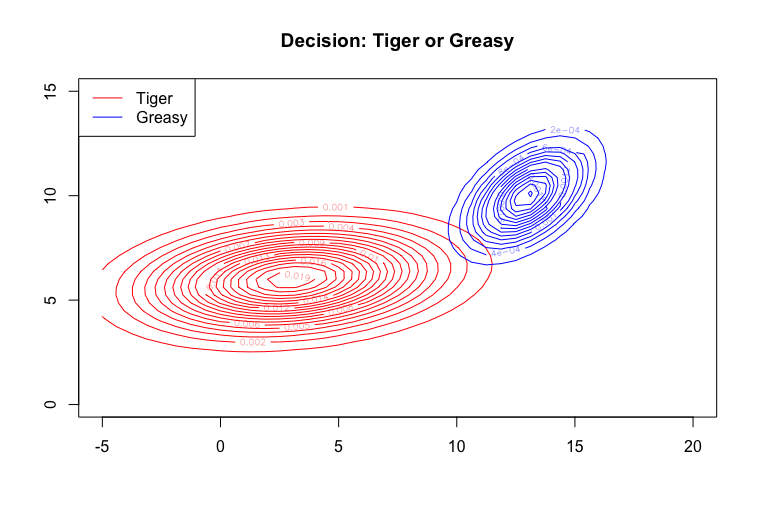
\includegraphics[width = 0.65\textwidth]{DB.png}
\end{figure*}

\qquad We draw the contour of the two distribution, and the decision bondary.

\begin{figure*}[h]
\centering
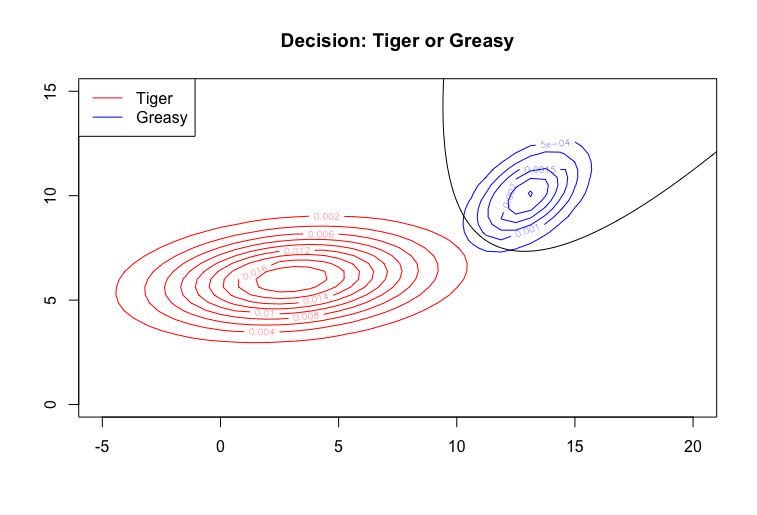
\includegraphics[width = 0.65\textwidth]{TG.png}
\end{figure*}

\subsection*{c)}

\qquad The left part is the region where a fish should be classified as a tiger, and the right part is the reigion where the fish should be classified as a greasy.

\end{flushleft}
\end{document}